\subsection{Similarity Between Two Fuzzy Sets}
\label{sec:fuzzySim}
Crisp set is a special case of fuzzy set, with \{0,1\} as the range of its characteristic function, rather than [0,1]. In other words, fuzzy set is a generalization of crisp set. According to this perspective, we generalized the similarity between fuzzy sets from definition \ref{CrispSim}, which is similarity between crisp sets.

\begin{defin}\textbf{Similarity between two fuzzy sets}\label{FuzzySim}
Let $U$ be an universe of discourse, and $\mu_{A}$, $\mu_{B}$ be characteristic functions of fuzzy sets $A$, $B$ respectively. If the $U$ is finite, with size of $n$, then the similarity between set $A$ and $B$ is defined as,
\begin{equation}\label{FSFinite}
Sim(A,B) =1- \frac{\sum_{i=1}^{n} \lvert \mu_{A}(e_i) - \mu_{B}(e_i) \rvert}{n}
\end{equation}
If the universal set $U$ is countable infinite, then the similarity between set $A$ and $B$ is defined as,
\begin{equation}\label{FSInfinite}
Sim(A,B) =1- \frac{\int_{x_{low}}^{x_{up}}\lvert \mu_{A}(x) - \mu_{B}(x) \rvert\, \mathrm{d}x}{\int_{x_{low}}^{x_{up}}\mathrm{d}x}
\end{equation}
\end{defin}
\begin{ex}
Two fuzzy sets are represented as two fuzzy functions as follows,
\[
  \mu_{A}(x) = \left\{ 
  \begin{array}{l l}
    e^{x} & \quad x \in [-2,0]\\
    1 & \quad x \in [0,1]\\
    -x+2 & \quad x \in [1,2]\\
  \end{array} \right.
\]

\[
  \mu_{B}(x) = \left\{ 
  \begin{array}{l l}
    - \frac{x}{2} & \quad x \in [-2,0]\\
    sin x & \quad x \in [0,2]\\
   \end{array} \right.
\]

\begin{figure}[h!]

\begin{center}
%\pagestyle{empty}
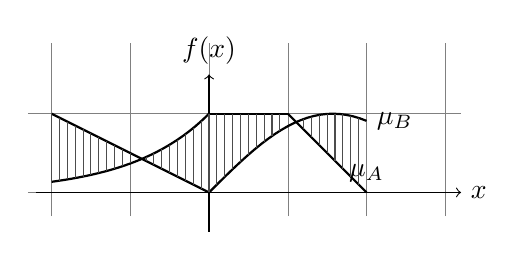
\begin{tikzpicture}

% defining the first function: the left, the middle, and the right part
\def\fonel{plot (\x, {exp(\x)})};
\def\fonem{plot (\x, {1})}; 
\def\foner{plot (\x, {-1*\x + 2})}; 

% defining the second function
\def\ftwol{plot (\x, {-0.5*\x})};
\def\ftwor{plot (\x, {sin(\x r)})};


% drawing the grid
\draw[very thin,color=gray] (-2.3,-0.3) grid (3.2,1.9);

% drawing the axes
\draw[->] (-2.2,0) -- (3.2,0) node[right] {$x$}; 
\draw[->] (0,-0.5) -- (0,1.5) node[above] {$f(x)$};



% drawing thw first function
\draw[color=black, thick, domain=-2:0] \fonel; 
\draw[color=black, thick, domain=0:1] \fonem;
\draw[color=black, thick, domain=1:2] \foner node[right, above] {$\mu_{A}$};

% drawing the second function
\draw[color=black, thick, domain=-2:0] \ftwol ;
\draw[color=black, thick, domain= 0:2] \ftwor node[right] {$\mu_{B}$};

% drawing the filler between functions
\foreach \x in {-2, -1.9, ..., -0.9} 
  \draw[color=black!70] (\x,0 |- 0,{-0.5*\x}) -- (\x,0 |- 0,{exp(\x)});
\foreach \x in {-0.8, -0.7, ..., 0} 
  \draw[color=black!70] (\x,0 |- 0,{exp(\x)}) -- (\x,0 |- 0,{-0.5*\x});
\foreach \x in {0, 0.1, ..., 1} 
  \draw[color=black!70] (\x,0 |- 0,{1}) -- (\x,0 |- 0,{sin(\x r)});
\foreach \x in {1.2, 1.3, ..., 2.0} 
  \draw[color=black!70] (\x,0 |- 0,{sin(\x r)}) -- (\x,0 |- 0,{-1*\x + 2});

\end{tikzpicture}

\end{center}
\caption{similarity between fuzzy sets $\mu_{A}$ and $\mu_{B}$}
\label{fig:Similarity between continuous functions}
\end{figure}

Then the distance between $\mu_{A}$ and $\mu_{B}$ is the average area of the grey part in Figure \ref{fig:Similarity between continuous functions}, according to formula \eqref{FSInfinite} in definition \ref{FuzzySim}.
\end{ex}